
% ----------------------------------------------------------------------
%  Set the document class
% ----------------------------------------------------------------------
\documentclass[11pt,a4paper,twoside]{article}

% ----------------------------------------------------------------------
% Define external packages, language, margins, fonts and new commands
% ----------------------------------------------------------------------
%\input{preamble} 
\usepackage[utf8]{inputenc}   % <<<<< Linux
\usepackage[english]{babel} % <<<<< English
\usepackage{notoccite}
\usepackage[skip=0.5\baselineskip]{caption}
\hyphenation{GTKWave}
\usepackage{listings}
\usepackage[all]{nowidow}

%blind text
\usepackage{lipsum}

\usepackage{comment} % comment out large bodies of text

\usepackage{graphicx}
\graphicspath{ {./} {../../figlib/} }
\def\FontLn{% 16 pt normal
  \usefont{T1}{phv}{m}{n}\fontsize{16pt}{16pt}\selectfont}
\def\FontLb{% 16 pt bold
  \usefont{T1}{phv}{b}{n}\fontsize{16pt}{16pt}\selectfont}
\def\FontMn{% 14 pt normal
  \usefont{T1}{phv}{m}{n}\fontsize{14pt}{14pt}\selectfont}
\def\FontMb{% 14 pt bold
  \usefont{T1}{phv}{b}{n}\fontsize{14pt}{14pt}\selectfont}
\def\FontSn{% 12 pt normal
  \usefont{T1}{phv}{m}{n}\fontsize{12pt}{12pt}\selectfont}

% Use Arial font as default
%
\renewcommand{\rmdefault}{phv}
\renewcommand{\sfdefault}{phv}
\usepackage{geometry}	
\geometry{verbose,tmargin=2.5cm,bmargin=2.5cm,lmargin=2.5cm,rmargin=2.5cm}

%\usepackage{setspace}
%\renewcommand{\baselinestretch}{1.5}

\usepackage[pdftex]{hyperref} % enhance documents that are to be
                              % output as HTML and PDF
\hypersetup{colorlinks,       % color text of links and anchors,
                              % eliminates borders around links
%            linkcolor=red,    % color for normal internal links
            linkcolor=black,  % color for normal internal links
            anchorcolor=black,% color for anchor text
%            citecolor=green,  % color for bibliographical citations
            citecolor=black,  % color for bibliographical citations
%            filecolor=magenta,% color for URLs which open local files
            filecolor=black,  % color for URLs which open local files
%            menucolor=red,    % color for Acrobat menu items
            menucolor=black,  % color for Acrobat menu items
%            pagecolor=red,    % color for links to other pages
            pagecolor=black,  % color for links to other pages
%            urlcolor=cyan,    % color for linked URLs
            urlcolor=black,   % color for linked URLs
	          bookmarks=true,         % create PDF bookmarks
	          bookmarksopen=false,    % don't expand bookmarks
	          bookmarksnumbered=true, % number bookmarks
	          pdftitle={report},
            pdfauthor={Conanga, H.P.},
%            pdfsubject={Thesis Title},
%            pdfkeywords={Thesis Keywords},
            pdfstartview=FitV,
            pdfdisplaydoctitle=true}

\usepackage[numbers,sort&compress]{natbib} % <<<<< References in numbered list [1],[2],...
\usepackage{subcaption} 
\usepackage{mdframed}
\usepackage{amsmath} % facilitates writing math formulas and improves the typographical quality of their output

%%%%%%%%%%%%%%%%%%%%%%%%%%%%%%%%%%%%%%%%%%%%%%%%%%%%%%%%%%%%%%%%%%%%%%%%
%     Begin Document                                                   %
%%%%%%%%%%%%%%%%%%%%%%%%%%%%%%%%%%%%%%%%%%%%%%%%%%%%%%%%%%%%%%%%%%%%%%%%


\begin{document}

% Set plain page style (no headers, footer with centered page number)
\pagestyle{plain}

% Set roman numbering (i,ii,...) before the start of chapters
%\pagenumbering{roman}

% ----------------------------------------------------------------------
%  Cover page
% ----------------------------------------------------------------------
%%%%%%%%%%%%%%%%%%%%%%%%%%%%%%%%%%%%%%%%%%%%%%%%%%%%%%%%%%%%%%%%%%%%%%%%
%                                                                      %
%     File: Thesis_FrontCover.tex                                      %
%     Tex Master: Thesis.tex                                           %
%                                                                      %
%     Author: Andre C. Marta                                           %
%     Last modified :  2 Jul 2015                                      %
%                                                                      %
%%%%%%%%%%%%%%%%%%%%%%%%%%%%%%%%%%%%%%%%%%%%%%%%%%%%%%%%%%%%%%%%%%%%%%%%

\thispagestyle {empty}

% IST Logo - Signature A
% parameters: bb=llx lly urx ury (bounding box), width=h_length, height=v_length, angle=angle, scale=factor, clip=true/false, draft=true/false. 
%\includegraphics[bb=9.5cm 11cm 0cm 0cm,scale=0.29]{IST_A_CMYK_POS}

\begin{center}
%
% Figure (Image or plot)
\vspace{1.0cm}
% height = 50 mm
%\includegraphics[height=50mm]{Figures/Airbus_A350.jpg}

% Title, author and degree
\vspace{1cm}
{\FontLb Circuit Theory and Electronics Fundamentals} \\ % <<<<< EDIT TITLE
\vspace{1cm}
{\FontSn Department of Electrical and Computer Engineering, Técnico, University of Lisbon} \\ % <<<<< EDIT COURSE
\vspace{1cm}
{\FontSn Example Laboratory Report} \\
\vspace{1cm}
{\FontSn February 27, 2021} \\ % <<<<< EDIT DATE (corresponds to date of oral examination)
%
\end{center}



% ----------------------------------------------------------------------
% Dedication page (optional)
% ----------------------------------------------------------------------
%\input{dedication} 
%\cleardoublepage

% ----------------------------------------------------------------------
%  Acknowledgments (optional)
% ----------------------------------------------------------------------
%\input{acknowledgements}
%\cleardoublepage

% ----------------------------------------------------------------------
%  Abstract (both in English and Portuguese)
% ----------------------------------------------------------------------
%\input{resumo} 
%\cleardoublepage

%\input{abstract} 

% ----------------------------------------------------------------------
%  Table of contents, list of tables, list of figures and nomenclature
% ----------------------------------------------------------------------

% Table of contents
%
\tableofcontents

% List of tables
%\addcontentsline{toc}{section}{\listtablename}
%\listoftables
%\cleardoublepage 

% List of figures
%\addcontentsline{toc}{section}{\listfigurename}
%\listoffigures
%\cleardoublepage 

% Set arabic numbering (1,2,...) after preface
%
%\setcounter{page}{1}
%\pagenumbering{arabic}

% ----------------------------------------------------------------------
%  Body
% ----------------------------------------------------------------------

\section{Introduction}
\label{sec:introduction}

% state the learning objective 
The objective of this laboratory assignment is to study a resistive circuit containing linear components, such as resistors ($R_i$), independent (circle shaped) and dependent (rhombus shaped) voltage ($V$) and current ($I$) sources, as seen in Figure~\ref{fig:esq}. To this end, the currents in every branch and the nodal voltages of the circuit are evaluated, using both the mesh and the nodal methods. For illustration and analysis purposes, the nodes are identified by the red numbers, the elementary meshes by the red subscript letters (in $I_i$) and the arrows point in the conventionalized current way.

In Section \ref{sec:analysis}, a theoretical analysis is presented, using said mesh (in Subsection \ref{subsec:mesh}) and nodal (in Subsection \ref{subsec:node}) methods. In Section~\ref{sec:simulation}, the circuit is analyzed by simulation, using the Ngspice software.
The results are compared in Section \ref{sec:simulation}. The conclusions of this study are outlined in
Section \ref{sec:conclusion}.



\begin{figure}[h] \centering
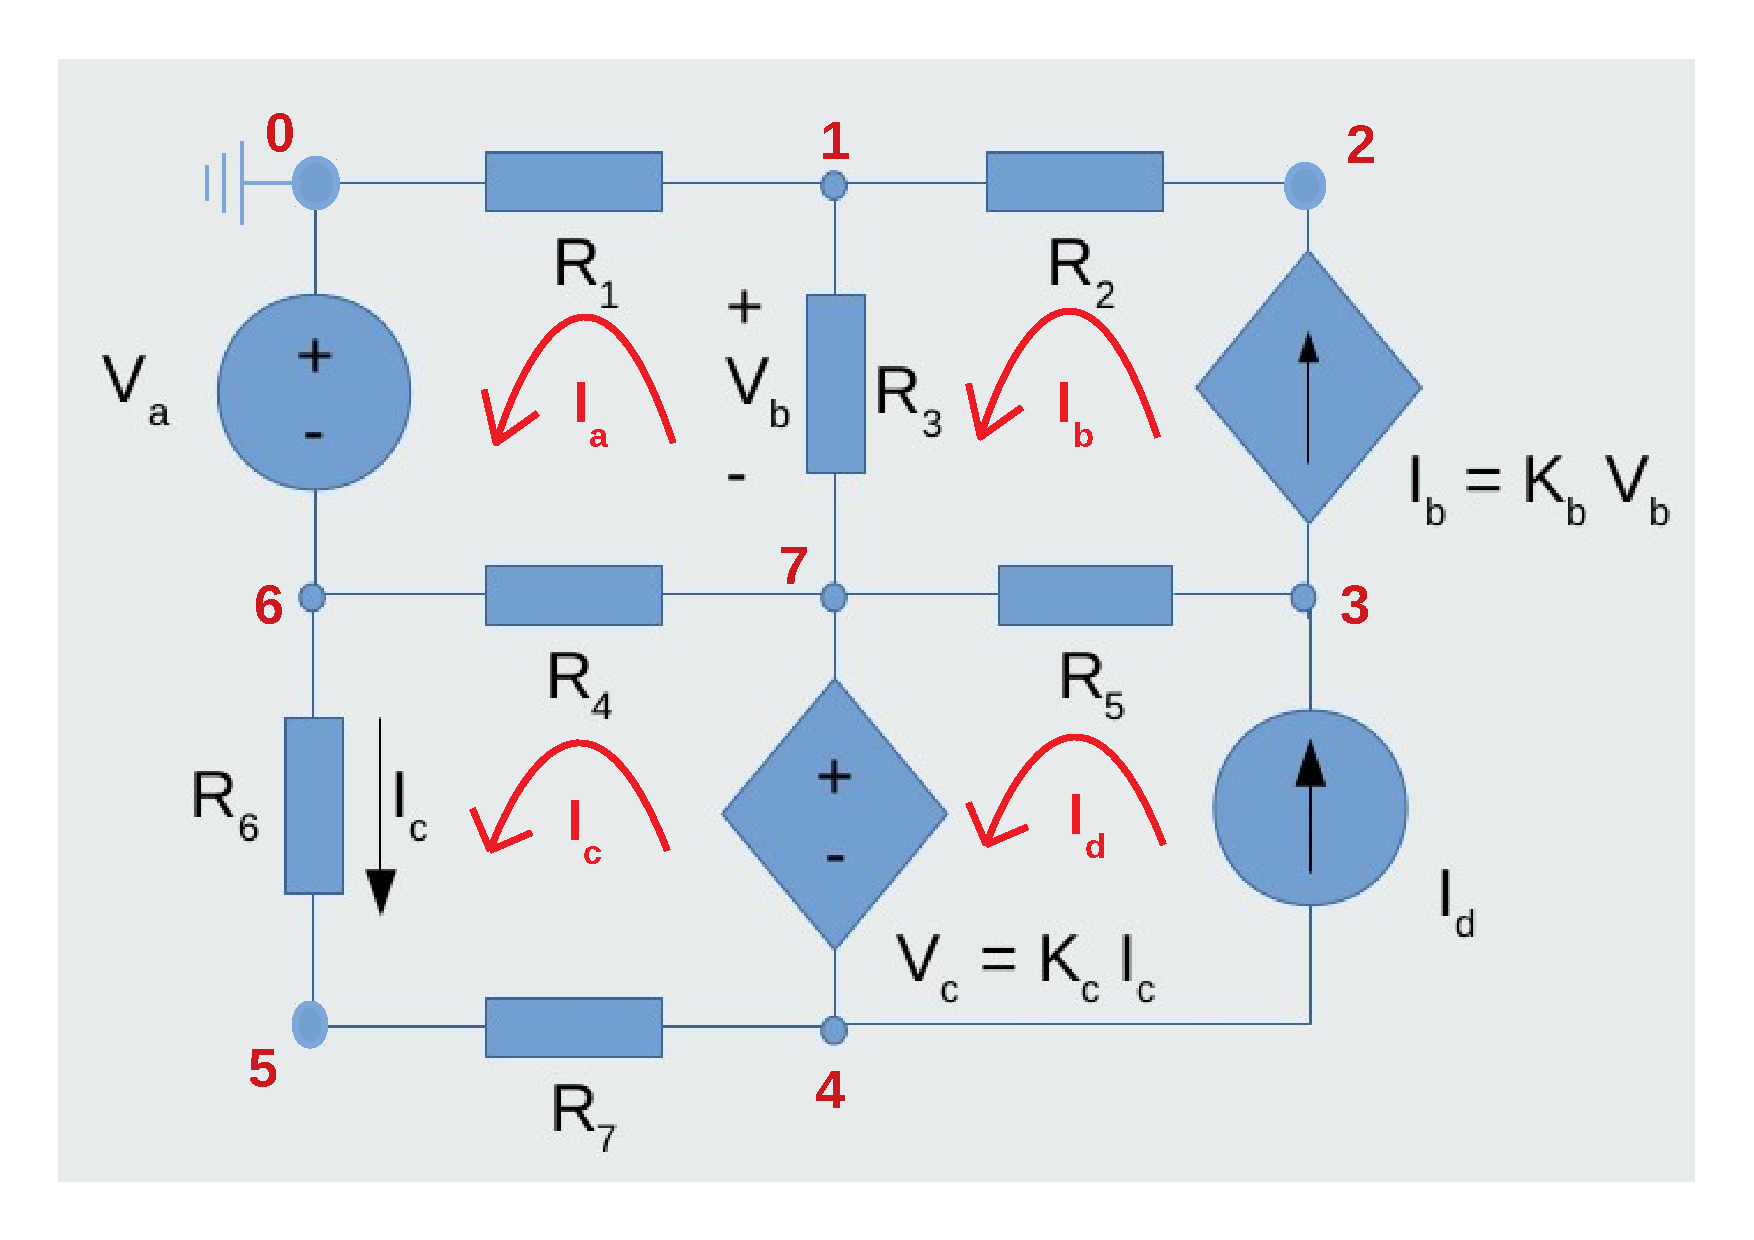
\includegraphics[width=0.8\linewidth]{esq_circ.pdf}
\caption{Resistive circuit.}
\label{fig:esq}
\end{figure}



\section{Theoretical Analysis}
\label{sec:analysis}

\subsection{Mesh Method}
\label{subsec:mesh}

The circuit consists of four elementary meshes: (a), (b), (c) and (d), respectively associated with mesh currents $I_a$, $I_b$, $I_c$ and $I_d$ (seen in Figure~\ref{fig:esq}) and with equations Eq. (a), Eq. (b),  Eq. (c) and Eq. (d): these are the result of the direct application of the mesh method and they are respectively presented as the first four equations in the system of linear equations \ref{eq:mesh_syst}.

Since the current in the dependent current source is a function of $V_b$, a four equation system would be undetermined. Hence, $V_b$ is equated as a function of the mesh currents passing through $R_3$, in the fifth equation of the system \ref{eq:mesh_syst}. 

\begin{equation}
    \begin{cases}
      I_a \cdot R_1 + V_a + I_a \cdot R_4 - I_c \cdot R_4 + I_a \cdot R_3 - I_b \cdot R_3 = 0\\
      I_b = K_b \cdot V_b\\
      I_c \cdot R_4 - I_a \cdot R_4 + I_c \cdot R_6 + I_c \cdot R_7 - K_c \cdot I_c = 0\\
      I_d = I_d\\
      V_b = R_3 \cdot ( I_b - I_a )\\
    \end{cases}\,.
    \label{eq:mesh_syst}
\end{equation}

This system can be presented in matrix form as in~\ref{eq:mesh_matrix}

\begin{gather}
    \begin{bmatrix} 
      \ (R_1 + R_4 + R_3) & -R_3 & -R_4 & 0 & 0 \\ 0 & 1 & 0 & 0 & -K_b \ \\ -R_4 & 0 & (R_4 + R_6 + R_7 - K_c) & 0 & 0 \\ 0 & 0 & 0 & 1 & 0 \\ R_3 & -R_3 & 0 & 0 & 1
    \end{bmatrix}
    \begin{bmatrix}
      \ I_a \ \\ I_b \\ I_c \\ I_d \\ V_b 
    \end{bmatrix}
    =
    \begin{bmatrix}
      \ -V_a \ \\ 0 \\ 0 \\ I_d \\ 0 
    \end{bmatrix}
    \label{eq:mesh_matrix}
\end{gather}

and computed in Octave scripts, from which the Table~\ref{tab:op1} is obtained.

\begin{table}[h]
  \centering
  \begin{tabular}{|l|r|}
    \hline    
    {\bf Name} & {\bf Value [A or V]} \\ \hline
    Ia & -0.000246\\ \hline 
Ib & -0.000257\\ \hline 
Ic & 0.000968\\ \hline 
Id & 0.001004\\ \hline
  \end{tabular}
  \caption{Operating point. A variable preceded by @ is of type {\em current}
    and expressed in Ampere; other variables are of type {\it voltage} and expressed in
    Volt.}
  \label{tab:op1}
\end{table}

As learned in theory classes and understood from Figure~\ref{fig:esq}, the current in a branch is a function of the mesh currents the branch is associated with. If the branch is associated with only one mesh current, then its current equals the mesh current. That is not the case for the branches formed by the $R_3$, $R_4$, $R_5$ and $V_c$ components. To determined those currents, the equations \ref{eq:R_3}, \ref{eq:R_4}, \ref{eq:R_5}, and \ref{eq:V_c} are used.

\begin{equation}
  Ir3=I_a-I_b
  \label{eq:R_3}
\end{equation}
in which $Ir3$ is the current flowing from node 7 to 1.
\begin{equation}
  Ir4=I_a-I_c
  \label{eq:R_4}
\end{equation}
in which $Ir4$ is the current flowing from node 6 to 7.

\begin{equation}
  Ir5=I_d-I_b
  \label{eq:R_5}
\end{equation}
in which $Ir5$ is the current flowing from node 3 to 7.

\begin{equation}
  Ivc=I_d-I_c
  \label{eq:V_c}
\end{equation}
in which $Ivc$ is the current flowing from node 7 to 4.

The results obtained with Octave are presented in Table~\ref{tab:op2}.

\begin{table}[h]
  \centering
  \begin{tabular}{|l|r|}
    \hline    
    {\bf Name} & {\bf Value [A or V]} \\ \hline
    Ir3 & 0.000011\\ \hline 
Ir4 & -0.001214\\ \hline 
Ir5 & 0.001261\\ \hline 
Ivc & 0.000036\\ \hline
  \end{tabular}
  \caption{Operating point. A variable preceded by @ is of type {\em current}
    and expressed in Ampere; other variables are of type {\it voltage} and expressed in
    Volt.}
  \label{tab:op2}
\end{table}



\subsection{Node Method}
\label{subsec:node}


The circuit consists of 8 nodes: 0 (ground), 1, 2, 3, 4, 5, 6 and 7, respectively associated with nodal voltages $V_0$, $V_1$, $V_2$, $V_3$, $V_4$, $V_5$, $V_6$ and $V_7$ (seen in Figure~\ref{fig:esq}). 

The nodal equations obtained with the nodal method pertain to the mentioned nodes as follows.
\\
\\
\textit{Node 0}:
\begin{equation}
  V_0=0
  \label{eq:N_0}
\end{equation}
\textit{Node 1}:
\begin{equation}
    (V_1 - V_0) \cdot G_1 + (V_1 - V_2) \cdot G_2 + V_b \cdot G_3 = 0
    \label{eq:N_1}
\end{equation}
\textit{Node 2}:
\begin{equation}
    (V_2 - V_1) \cdot G_2 - K_b \cdot V_b = 0
    \label{eq:N_2}
\end{equation}
\textit{Node 3}:
\begin{equation}
    (V_3 - V_7) \cdot G_5 - I_d + K_b \cdot V_b = 0
    \label{eq:N_3}
\end{equation}
\textit{Node 4}:
\begin{equation}
    I_c - Ivc + I_d = 0
    \label{eq:N_4_1}
\end{equation}
\begin{equation}
    V_4 = - V_c + V_7
    \label{eq:N_4_2}
\end{equation}
\textit{Node 5}:
\begin{equation}
  (V_5 - V_6) \cdot G_6 + (V_5 - V_4) \cdot G_7 = 0
  \label{eq:N_5}
\end{equation}
\textit{Node 6}:
\begin{equation}
    V_6 = - V_a
  \label{eq:N_6}
\end{equation}
\textit{Node 7}:
\begin{equation}
  Ivc + (V_7 - V_3) \cdot G_5 + (V_7 - V_2) \cdot G_3 + (V_7 - V_6) \cdot G_4 = 0
  \label{eq:N_7}
\end{equation}

To obtain a determined linear system of equations, three other equations are added. Both $V_b$ and $I_c$ need to be written as a function of nodal voltages, as shown in equations \ref{eq:Add_Vb} and \ref{eq:Add_Ic}. $V_C$ should be equated as shown in Figure \ref{fig:esq} and as written in equation \ref{eq:Add_Vc}.

\begin{equation}
    V_b = V_1 - V_7
    \label{eq:Add_Vb}
\end{equation}

\begin{equation}
    V_5 + I_c \cdot R_6 = V_6 \Leftrightarrow I_c = (V_6 - V_5) \cdot G_6
    \label{eq:Add_Ic}
\end{equation}

\begin{equation}
    V_c = K_c \cdot I_c
    \label{eq:Add_Vc}
\end{equation}


Applying the added equations \ref{eq:Add_Vb}, \ref{eq:Add_Ic} and \ref{eq:Add_Vc} to the previously presented nodal 
equations, the system of linear equations (produced in matrix form) is \ref{eq:nodal_matrix}

\begin{gather}
  \begin{bmatrix} 
    (G_1 + G_2 + G_3) & -G_2 & 0 & 0 & 0 & 0 & -G_3 & 0 \\ -G_2 - K_b & G_2 & 0 & 0 & 0 & 0 & K_b & 0 \\ K_b & 0 & G_5 & 0 & 0 & 0 & (-K_b-G_5) & 0 \\ 0 & 0 & 0 & -G_7 & (G_6+G_7) & -G_6 & 0 & 0 \\ 0 & 0 & 0 & 1 & (-K_c \cdot G_6) & (K_c \cdot G_6) & -1 & 0 \\ 0 & 0 & 0 & 0 & 0 & 1 & 0 & 0 
  \end{bmatrix}
  \begin{bmatrix}
    V_1 \\ V_2 \\ V_3 \\ V_4 \\ V_5 \\ V_6 \\ V_7 \\ I_t
  \end{bmatrix}
  =
  \begin{bmatrix}
    0 \\ 0 \\ I_d \\ 0 \\ 0 \\ -V_a \\ -I_d \\ 0
  \end{bmatrix}
  \label{eq:nodal_matrix}
\end{gather}


Lastly, an Octave script running \ref{eq:nodal_matrix} is used to obtain the results in Table~\ref{tab:op3}.


\begin{table}[h]
  \centering
  \begin{tabular}{|l|r|}
    \hline    
    {\bf Name} & {\bf Value [A or V]} \\ \hline
    V1 & -0.249911\\ \hline 
V2 & -0.778383\\ \hline 
V3 & 3.700284\\ \hline 
V4 & -8.073949\\ \hline 
V5 & -7.067894\\ \hline 
V6 & -5.113245\\ \hline 
V7 & -0.214558\\ \hline 
Ivc & 0.000036\\ \hline
  \end{tabular}
  \caption{Operating point. A variable preceded by @ is of type {\em current}
    and expressed in Ampere; other variables are of type {\it voltage} and expressed in
    Volt.}
  \label{tab:op3}
\end{table}







\section{Simulation Analysis}
\label{sec:simulation}

To accurately simulate the circuit in ngspice, precaution is needed with the positive and negative nodes associated with each component, since an error in these parameters would cause currents and voltage sources operating in the wrong direction.

It's important to add that due to a peculiarity of the program, we couldn't get the current in the resistance $R_5$ as a reference for the current dependent voltage source. To solve that, we created a dummy source($V_8$ with value 0) in that branch so that the program could get a valid read. That is the reason why in the table \ref{tab:op} we have $V_8$ with the value that $V_6$.

Table~\ref{tab:op} shows the simulated operating point results for the circuit
under analysis were is present the values of the current through all components as well as the voltages in each node. 


\begin{table}[h]
  \centering
  \begin{tabular}{|l|r|}
    \hline    
    {\bf Name} & {\bf Value [A or V]} \\ \hline
    @gb[i] & -1.85722e-03\\ \hline
@id[current] & 1.003968e-03\\ \hline
@r1[i] & -1.85714e-03\\ \hline
@r2[i] & 1.857222e-03\\ \hline
@r3[i] & -8.11657e-08\\ \hline
@r4[i] & 7.994898e-04\\ \hline
@r5[i] & -2.86119e-03\\ \hline
@r6[i] & -1.05765e-03\\ \hline
@r7[i] & -1.05765e-03\\ \hline
v(1) & -1.88731e+00\\ \hline
v(2) & -5.70404e+00\\ \hline
v(3) & 6.994799e+00\\ \hline
v(4) & -1.87847e+00\\ \hline
v(5) & -2.97765e+00\\ \hline
v(6) & -5.11325e+00\\ \hline
v(7) & -1.88706e+00\\ \hline
v(8) & -5.11325e+00\\ \hline

  \end{tabular}
  \caption{Simulation results; A variable preceded by @ is of type {\em current}
    and expressed in Ampere; other variables are of type {\it voltage} and expressed in
    Volt.}
  \label{tab:op}
\end{table}


Comparing these results with the previous tables given with octave, it can easily be seen that our results match, reasons from which will be mentioned in the next section.
Diferences in the signal of some currents are due to assumptions previosly made in the direction of 
the current flow.


\section{Conclusion}
\label{sec:conclusion}

In this laboratory assignment the objective of analysing an RC circuit has been
achieved. Static, time and frequency analyses have been performed both
theoretically using the Octave maths tool and by circuit simulation using the
Ngspice tool. The simulation results matched the theoretical results
precisely. The reason for this perfect match is the fact that this is a
straightforward circuit containing only linear components, so the theoretical
and simulation models cannot differ. For more complex components, the
theoretical and simulation models could differ but this is not the case in this
work.



%\cleardoublepage

% ----------------------------------------------------------------------
%  Bibliography
% ----------------------------------------------------------------------
%\addcontentsline{toc}{section}{\bibname}
%\bibliographystyle{abbrvunsrtnat} % <<<<< SELECT IF USING REFERENCES BY NUMBER (CITATION ORDER)
%\bibliography{../../../BIBfile.bib}

% ----------------------------------------------------------------------
\end{document}
% ----------------------------------------------------------------------

